\documentclass[a4paper,11pt]{article}
\usepackage[a4paper]{geometry}
\usepackage{hyperref}
\usepackage{syntax}
\usepackage{listings}
\lstset{language=C}
\usepackage{parskip}
\usepackage{setspace}
\onehalfspace
\usepackage{subfig}
\usepackage{graphicx}
\DeclareGraphicsExtensions{.pdf,.png,.jpg}

\hypersetup{
    colorlinks,
    citecolor=black,
    filecolor=black,
    linkcolor=black,
    urlcolor=black
}

\author{Christian Manning -- p0928544x\\
De Montfort University}
\title{IMAT3451 -- Final Year Project\\
    Dynamic Data Structure Visualisation\\
    User Documentation
}
\date{April 2012}

\begin{document}
\maketitle

\tableofcontents
\listoffigures

\clearpage

\section{Introduction}

The Dynamic Data Structure Visualisation (DDSV) application aims to provide help to students who are learning to program.
The focus of this application is on the concept of pointers; specifically, how they are used to build data structures.

It does this by utilising a graphical user interface (GUI) to provide a visualisation containing graphical representations of abstract data types and pointers to them.
This facilitates the visual construction of a data structure, which can then be manipulated to simulate algorithmic operations.

Another interface to this application utilises the expressiveness of a programming language from the GUI in the form of an interpreter.
The language accepted by this interpreter, is a small subset of the C programming language which has quite a low level model and so pointers are exposed to the user more readily.
With this interpreter, C code can then be visualised graphically, allowing the user to learn 


\section{Interpreted Language}

\subsection{Specification}

This is the formal grammar specification of the interpreted language using an Extended Backus-Naur Form (EBNF)-like notation, with some brief descriptions.
Each entry is referred to as a grammar \textit{rule}.

Key:\\
\begin{tabular}{|c|l|}
 \hline
 \textbf{Symbols} & \textbf{Description} \\ \hline
 \verb+<a>+ & \verb+a+ is a non-terminal \\ \hline
 \verb+a+ ::= \verb+b+ & \verb+a+ is defined as a rule with \verb+b+ as its singular constituent \\ \hline
 \verb+a+ \verb+b+ & \verb+a+ followed by \verb+b+ \\ \hline
 (\verb+a+ \verb+b+) & Groups rules \verb+a+ and \verb+b+ together \\ \hline
 {\verb+a+} & Repeat \verb+a+ zero, one or more times \\ \hline
 [\verb+a+] & \verb+a+ is to be matched zero or one times. (Optional) \\ \hline
 \verb+a | b+ & \verb+a+ \textit{or} \verb+b+ \\ \hline
 \verb+-a+ & Do not match \verb+a+ \\ \hline
 `\verb+c+' & Character string \verb+c+ \\ \hline
 \%\verb+a+ & Comma separated list of \verb+a+ \\ \hline
 ; & End of rule \\ \hline
\end{tabular}


\noindent\textit{assign\_op} ::=
    `$=$'
    ;

\noindent\textit{logical\_or\_op} ::=
    `$||$'
    ;

\noindent\textit{logical\_and\_op} ::=
    `$\&\&$'
    ;

\noindent\textit{equality\_op} ::=
    `$==$'
    $|$ `$!=$'
    ;

\noindent\textit{relational\_op} ::=
    `$<$'
    $|$ `$\leq$'
    $|$ `$>$'
    $|$ `$\geq$'
    ;

\noindent\textit{additive\_op} ::=
    `$+$'
    $|$ `$-$'
    ;

\noindent\textit{multiplicative\_op} ::=
    `$*$'
    $|$ `$/$'
    ;

\noindent Listed above are the \textit{binary operators}, meaning they require two \textit{operands}. These are arithmetic and boolean operators.

\noindent\textit{unary\_op} ::=
    `$+$'
    $|$ `$-$'
    $|$ `$!$'
    $|$ `$*$'
    $|$ `$\&$'
    ;

\noindent\textit{Unary operators} require only one \textit{operand}.

\noindent\textit{struct\_op} ::=
    `$->$'
    $|$ `$.$'

\noindent\textit{Struct operators} are used to select members of a struct variable.
    
\noindent\textit{memory\_op} ::=
    `\verb+new+'
    
\noindent The \textit{new} operator is used for dynamically allocating memory.

\noindent\textit{keywords} ::=
    `\verb+true+' $|$ `\verb+false+' $|$ `\verb+if+' $|$ `\verb+while+' $|$ `\verb+struct+' $|$ `\verb+return+' $|$ `\verb+new+'
    ;

\noindent These are the \textit{keywords} which are reserved words and cannot be used outside of their required context.

\noindent\textit{types} ::=
    `\verb+void+' $|$ `\verb+int+' $|$ `\verb+bool+' ;
    
\noindent These are the predefined primitive \textit{types} that are used for declaring variables, etc.

\begin{grammar}
<identifier> ::=
	-(keywords | types) ,
	alpha | `\_' , \{ alpha | digit | `\_' \} ;
\end{grammar}
An \textit{identifier} must not be a \textit{keyword}, a primitive type or begin with a digit. It must start with an alphabetic character or an underscore (\_) to be optionally followed by zero or more alphabetic characters, digits or underscores. 

\begin{grammar}
        <assignment_expression> ::= <logical_OR_expression> [<unary_assign>];

        <allocation_expression> ::= <memory_op> <type_specifier>;

        <unary_assign> ::= <assign_op>\\
        (<allocation_expression> \alt <logical_OR_expression>);

        <logical_OR_expression> ::= <logical_AND_expression>\\
        \{<logical_or_op> <logical_AND_expression>\};

        <logical_AND_expression> ::= <equality_expression>\\
        \{<logical_and_op> <equality_expression>\};

        <equality_expression> ::= <relational_expression>\\
        \{<equality_op> <relational_expression>\};

        <relational_expression> ::= <additive_expression>\\
        \{<relational_op> <additive_expression>\};

        <additive_expression> ::= <multiplicative_expression>\\
        \{<additive_op> <multiplicative_expression>\};

        <multiplicative_expression> ::= <unary_expression>\\
        \{<multiplicative_op> <unary_expression>\};

        <unary_expression> ::=
                [<unary_op>]
               <postfix_expression>
            ;

        <struct_expr> ::= <struct_op> <identifier>;

        <postfix_expression> ::=
                <primary_expression>\\
               \{<struct_expr> \alt <postfix_op>\}
            ;

        <primary_expression> ::=
                int
            \alt   <identifier>
            \alt   bool
            \alt   `(' <logical_OR_expression> `)'
            ;
\end{grammar}
\textit{Assignment expression} is the catch-all expression rule.
This rule uses recursion so that it also takes into account operator precedence without additional algorithms.
Each of its constituent rules have a specific set of operators, each with their own precedence.

As can be seen from the top rule only one variable can be assigned at a time, whereas the rest can be composed of any of the others, allowing complex expressions to be formed.
Available primitive types for constants and variables are integer and boolean only.

An \textit{allocation expression} is one which allocates memory of a specified type to be assigned to a pointer.

\begin{grammar}
        <type_specifier> ::=
                <types>
            \alt   <struct_specifier>
            ;

        <declarator> ::= [`*'] <identifier>;
        
	<declaration> ::= <type_specifier> [<init_declarator>] `;';

        <init_declarator> ::= <declarator>
        [`=' <allocation_expression>
        \alt <logical_OR_expression>];


        <struct_member_declaration> ::= <type_specifier> <declarator> `;';

        <struct_specifier> ::=
                `struct' <identifier> [`{' \{<struct_member_declaration>\} `}';
\end{grammar}
The above lists the rule to match a \verb+struct+ definition, which may contain one or more member declarations.
A struct member declaration must not be initialised in any form.
Variable declarations may have a single initialisation from an expression.
The optional `*' denotes a pointer type.

\begin{grammar}
<statement_list> ::=
    \{<statement>\}
    ;

<statement> ::=
	<declaration>
    \alt   <assignment_expression> `;'
    \alt   <if_statement>
    \alt   <while_statement>
    \alt   <return_statement>
    \alt   <compound_statement>
    ;
\end{grammar}

Any of the above listed \textit{statements} can take the place of a $\langle statement\rangle$ instance.

\begin{grammar}
<if_statement> ::=
	`if'
       `('
       <logical_OR_expression>
       `)'
       <statement>
    ;
\end{grammar}

An \textit{if statement} is a conditional which will only execute its encompassed statement if a condition is evaluated as \verb+true+.
This condition can be anything that can be represented by a \textit{logical or expression}, which is any expression other than an assignment.

\begin{grammar}
<while_statement> ::=
	`while'
       '('
       <logical_OR_expression>
       `)'
       <statement>
    ;
\end{grammar}

The \textit{while statement} is a looping statement which will execute its enclosed statement for as long as its conditional \textit{logical or expression} evaluates to \verb+true+.

\begin{grammar}
<compound_statement> ::=
    '\{' [<statement_list>] '\}'
    ;
\end{grammar}
A \textit{compound statement} is an list of zero, one or many \textit{statements} enclosed in braces (`\{' \& `\}').
\begin{grammar}
<return_statement> ::=
	`return'
    [<logical_OR_expression>]
       `;'
    ;
\end{grammar}

\begin{grammar}
        <argument> ::=
                <type_specifier>
            <init_declarator>
            ;

        <function_definition> ::=
                <type_specifier>
            <declarator>\\
            `('
            [\%<argument>]
               `)'\\
            <compound_statement>
            ;

        <translation_unit> ::=
            \{  <statement>
            \alt   <function_definition>
            \}
            ;
\end{grammar}

The \textit{translation unit} consists of a list of both \textit{function} declarations and \textit{statement lists}. This is root of all that can be passed to the interpreter, i.e.\ everything must be entered in this form.

\subsection{Operator Precedence}
The following table shows the operator precedence of the interpreted language, from lowest to highest.

\begin{tabular}{| c | c | l |}
\hline
Precedence & Operator & Description \\ \hline
1 & = & Assignment \\ \hline
2 & $\parallel$ & Logical OR \\ \hline
3 & \&\& & Logical AND \\ \hline
4 & == & Equal \\
  & != & Not Equal \\ \hline
5 & $<$ & Less than \\
  & $\leq$ & Less than or equal to \\
  & $>$ & More than \\
  & $\geq$ & More than or equal to \\ \hline
6 & + (binary) & Addition \\
  & $-$ (binary) & Subtraction \\ \hline
7 & * & Multiplication \\
  & / & Division \\ \hline
8 & + (unary) & Plus \\
  & -- (unary) & Minus \\
  & ! & Not \\
  & $\&$ & Address of \\
  & * (unary) & Dereference \\ \hline
9 & $-$$>$ & Select element through pointer \\
  & . & Select element \\ \hline
\end{tabular}

The \verb+new+ operator does not have a particular precedence as it can only be used in assignments and declarations, effectively giving it a precedence higher than that of `=', though it is considered a special operator.

\subsection{Notes}

This language may be similar to C but there are some notable exceptions and omissions:
\begin{itemize}
 \item Only primitive types are \verb+int+ and \verb+bool+
 \item No arrays.
 \item No increment, decrement or arithmetic assignment (\verb/+=/, \verb+*=+, etc.) operators.
 \item No \verb+for+ loop.
 \item No \verb+else+ to accompany an \verb+if+ statement. A similar effect could be accomplished by negating the condition of the \verb+if+ statement.
 \item No recursive struct data types.
 \item Functions are currently parsed but not processed.
 \item Struct variables occupy an additional stack entry at its beginning.
\end{itemize}

Should the parser fail (i.e.\ fail to match any of the above rules), an error message is displayed in a dialog.
The information it provides will refer to the above rules informing of what rule was to be expected and also where it was expected (see figure \ref{fig:parseerror1}).
\begin{figure}[h!]
\centering
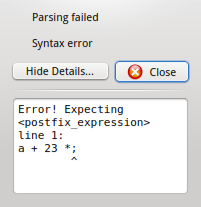
\includegraphics{parseerror1}
\caption{Syntax error.}
\label{fig:parseerror1}
\end{figure}
A similar error dialog will appear if an error occurs during processing after parsing (semantic analysis), though it attempts to be slightly more informative without needing to have the language specification handy.

\subsection{Examples}

\subsubsection{Variable Declaration}

\begin{lstlisting}
//declare an integer variable named "a"
int a;
//assignment on declaration
int b = 3;
//assignment from an expression
int c = b + 2;

//declare a pointer and assign it the address of a
int * p = &a;
*p = 51; // a == 51

//declare a pointer variable and allocate it some memory
int * x = new int;
//dereference and assign
*x = 123;
\end{lstlisting}

\subsubsection{Function Declaration}

\begin{lstlisting}
int factorial(int n) {
  if(n < 1)
    return 1;
  else
    return n * factorial(n-1);
}
\end{lstlisting}

\subsubsection{Struct Declaration}

\begin{lstlisting}
//Define a struct
struct point {
  int x;
  int y;
};

//Define and declare a struct variable in one statement
struct point {
  int x;
  int y;
} p1;

struct point * ptr = new struct point;
ptr->x = 42;
ptr->y = 24;
\end{lstlisting}

\subsubsection{Struct Instantiation}

\begin{lstlisting}
struct point p1;
p1.x = 4;
p1.y = 6;
\end{lstlisting}

\subsubsection{If Statement}

\begin{lstlisting}
int a = 123;

// performs the statement(s) only if the
// expression enclosed in () evaluates to true
if(a < 200) {
  a = a * 2;
}
// a == 246
\end{lstlisting}

\subsubsection{While Statement}

\begin{lstlisting}
int a = 123;

// performs the statement(s) repeatedly until the
// expression enclosed in () evaluates to false
while(a < 200) {
  a = a + 1;
}
// a == 200
\end{lstlisting}


\section{User Interface}

The user interface provides several ways to control and visualise program data.
Figure \ref{fig:mainwindow1} shows how the main UI appears when it is first opens, with nothing other than the basic UI elements displayed.
The large empty space here is the visualisation area.
This is where data items are displayed graphically once defined with the interpreter text input or added with the UI.
\begin{figure}[h!]
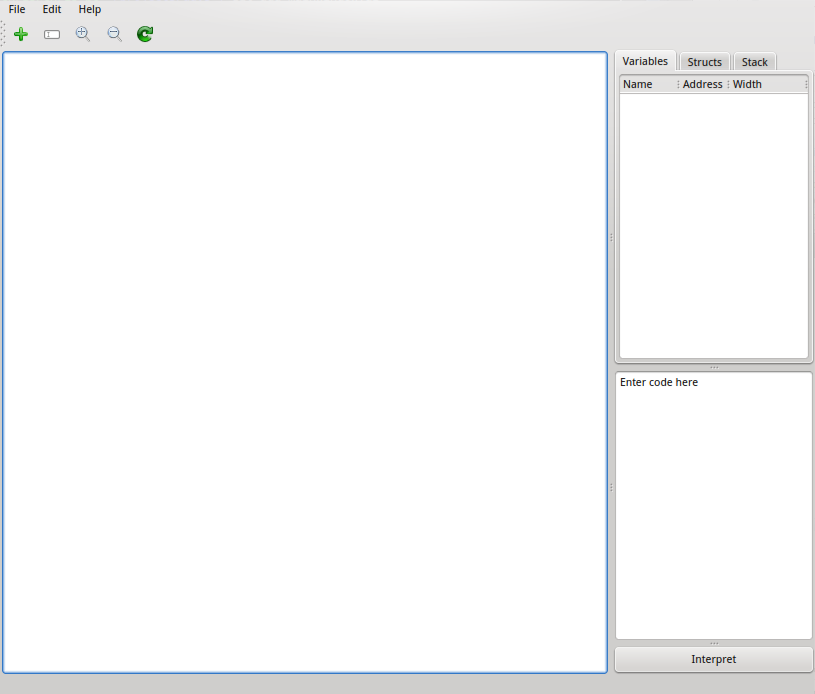
\includegraphics[width=\textwidth]{mainwindow1}
\caption{Empty main window.}
\label{fig:mainwindow1}
\end{figure}
In the upper-right of this screen-shot is a tabbed widget containing three tabs: Variables, Structs and Stack.
These contain informational (read-only) data concerning the underlying data structures and also to indicate the available struct types and their members.

Below the tabs is a text box, in which code for the C-like language defined above can be entered and then interpreted by using the wide push-button.

The tool bar pictured shows five icons which perform separate operations: add item, edit item, zoom in, zoom out and refresh view.
The mouse wheel also performs zooming functions, i.e.\ scroll up to zoom in and vice versa.
Once in a zoomed in state the visualisation area can be moved by clicking and dragging an empty space, or by using the scrollbars which will appear when applicable.

\subsection{Adding Variables}

Creating a variable instance to add to the visualisation can be accomplished in two ways, through the programming language interpreter (see previous examples) or by using the ``Add Item'' dialog.
This is activated by clicking either the `+' tool-bar button or the ``Add Item'' entry in the ``Edit'' menu.
Figure \ref{fig:addint1} shows this dialog with values entered for the declaration of a integer variable.
\begin{figure}[h!]
\centering
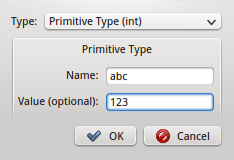
\includegraphics{addint1}
\caption{Add item dialog.}
\label{fig:addint1}
\end{figure}
If the entered values are at all invalid, the same dialog windows as those produced by entering text into the interpreter directly are utilised.

\subsection{Editing Variables}

Editing the values of variables can be achieved through the use of assignment expression statements using the interpreter, or the ``Edit Item'' dialog.
The graphic representing the variable intended to be edited must be selected, then either click the edit tool-bar button or the ``Edit Item'' entry in the ``Edit'' menu.
\begin{figure}[h!]
\centering
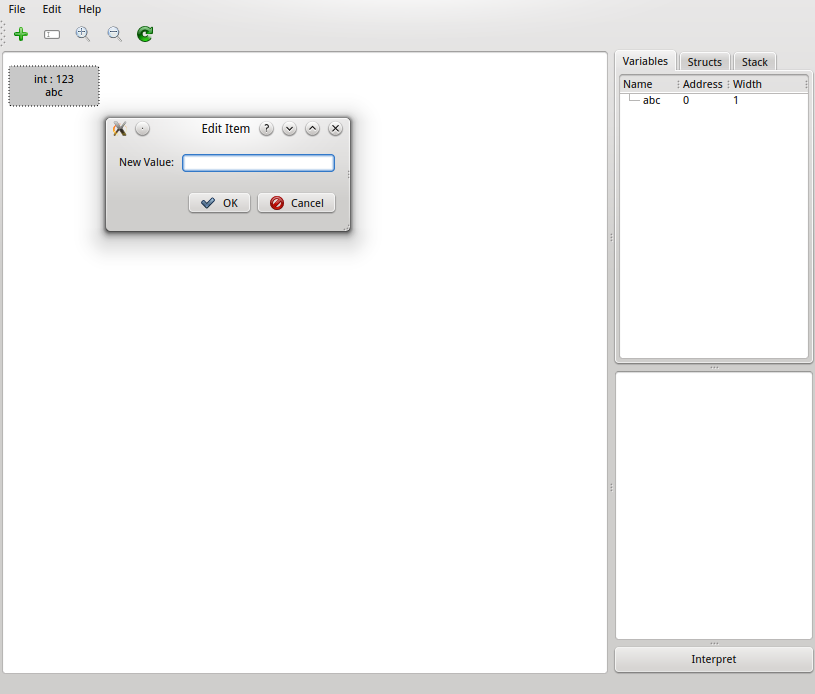
\includegraphics[trim=0 100mm 100mm 0,clip]{editint1}
\caption{Edit item dialog.}
\label{fig:editint1}
\end{figure}

\subsection{Stack Table}

The stack table provides information on the stack data structure which is operated on by the interpreter (see figures \ref{fig:stacktable1} and \ref{fig:stacktable2}).
\begin{figure}[h!]
\centering
\subfloat[Stack table]{\label{fig:stacktable1}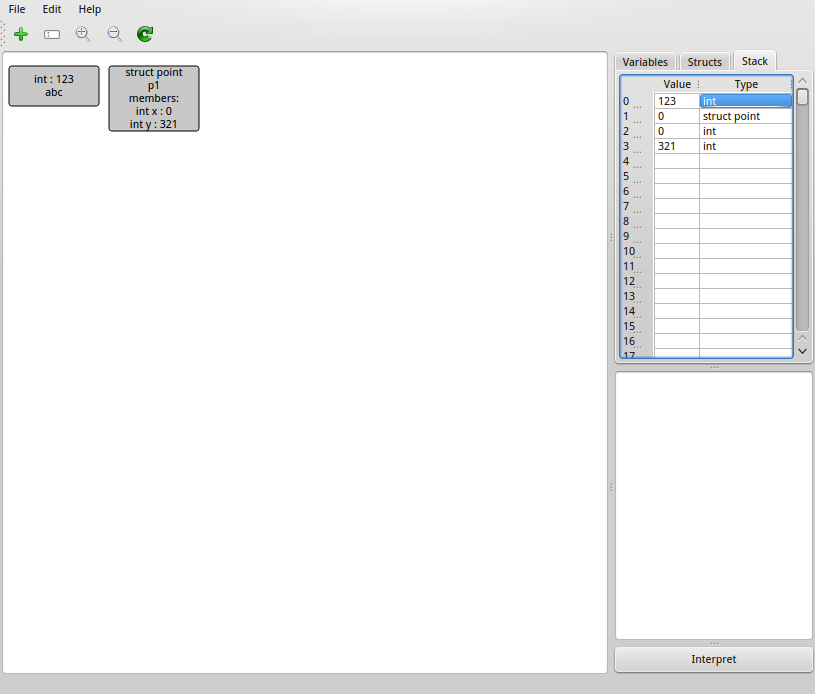
\includegraphics[trim=460 300 0 35,clip]{stacktable1}}
\hspace{10pt}
\subfloat[Items]{\label{fig:stacktable2}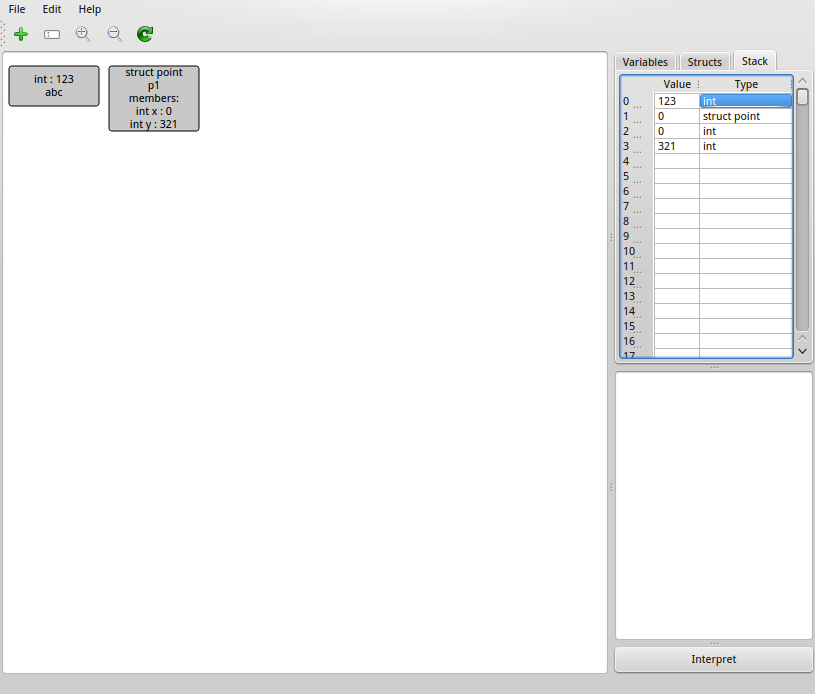
\includegraphics[trim=0 350 400 0,clip]{stacktable1}}
\caption{Stack table and items.}
\end{figure}
This information is useful in determining the memory layout of variables and struct data, and also to determine what value occupies at a particular stack address (the values in the left side headers are the stack addresses).

\subsection{Variable Table}

Figure \ref{fig:variabletable1} shows the variable table for the previous example.
\begin{figure}[h!]
\centering
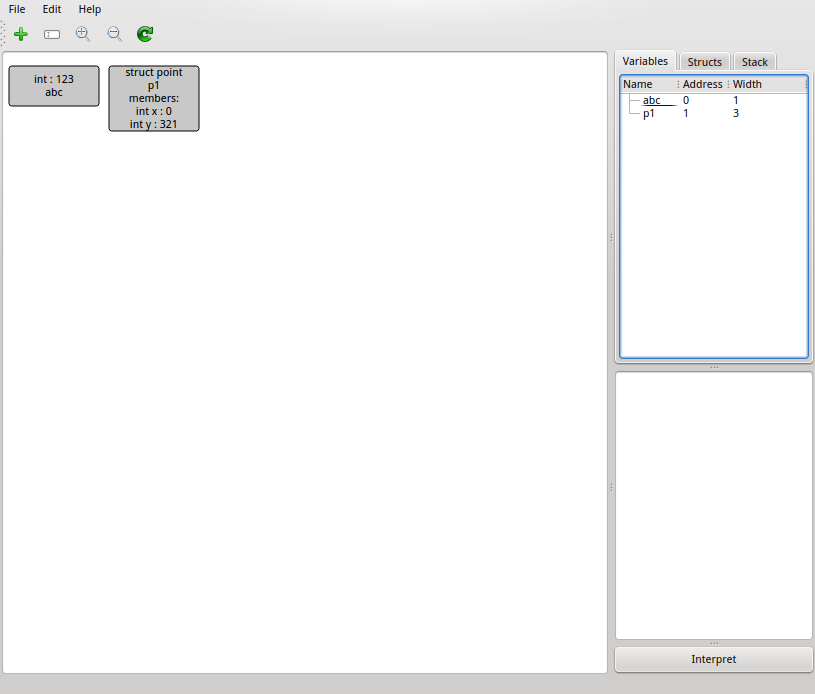
\includegraphics[trim=460 300 0 35,clip]{variabletable1}
\caption{Variable table.}
\label{fig:variabletable1}
\end{figure}
It shows each declared (or dynamically allocated) variable's name, stack address and the number of stack entries it occupies.
This, in combination with the stack table and struct tree described below, provides some important information with regard to diagnosing problems caused by pointers, much like a visual debugging interface.

\subsection{Struct Tree}

The struct tree, as shown in figure \ref{fig:structtree1}, displays each defined struct data type, with each of its members and their types as its children.
\begin{figure}[h!]
\centering
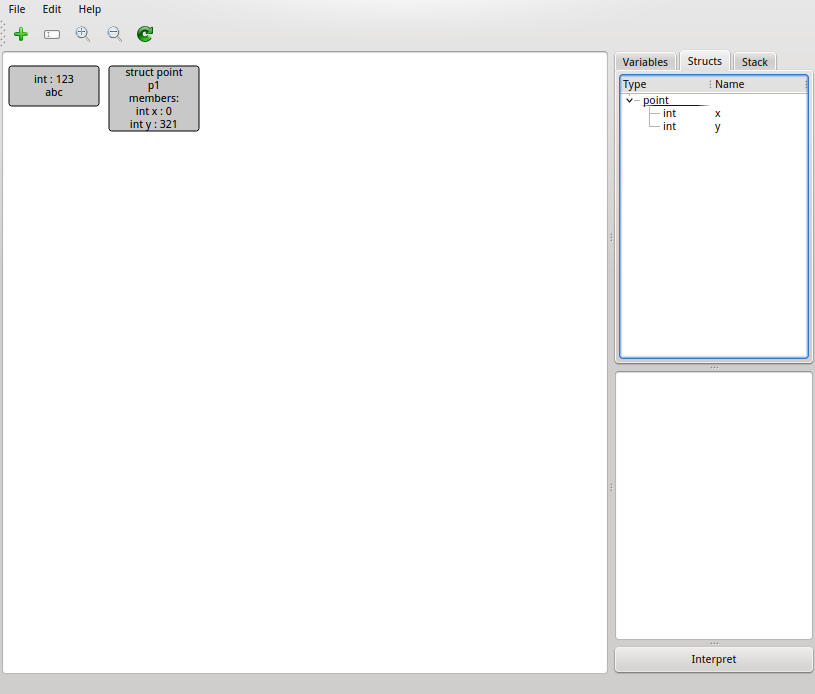
\includegraphics[trim=460 300 0 35,clip]{structtree1}
\caption{Struct tree.}
\label{fig:structtree1}
\end{figure}
This can be used with the stack table to determine which stack entries are for which member variable by both the order they appear in, and their type.

\end{document}
